\documentclass[letterpaper,12pt,twoside=false,DIV=11]{scrartcl}

%----------------------CONFIG---------------------------
%math packages
\usepackage{amsmath,amssymb,amsthm,units,unitsdef}

%bibliography style and citation style, bibstyles to use: plainnat, abbrvnat, unsrtnat, named, chicago
%otherwise numerical citationstyle will be used
%\usepackage[authoryear,round]{natbib}

\usepackage{longtable,tabularx,tabulary,multirow,lscape}
\usepackage[font={sl},format=plain,labelfont=bf]{caption}

% colors
\usepackage{color,colortbl}
\usepackage[dvipsnames]{xcolor}
\definecolor{darkblue}{HTML}{00354C}

\usepackage{booktabs}
%\usepackage{showkeys} % shows the labels above the references for

%easier development
\usepackage{ifpdf}

\ifpdf
    \usepackage[pdftex]{graphicx}
    \usepackage[]{pdfpages} %for including full pdf pages
    \usepackage[pdftex,
        bookmarks,
        bookmarksopen=true,
        bookmarksnumbered=true,
        pdfauthor={Reto Trappitsch},
        pdftitle={On the origin of elements in the Milky Way - Homework},
        colorlinks,
        linkcolor=darkblue,
        citecolor=darkblue,
        filecolor=black,
        urlcolor=darkblue,
        anchorcolor=black,
        menucolor=black,
        breaklinks=true,
        pageanchor=true, %for jumping to a page
        plainpages=false,
        pdfpagelabels=true]{hyperref}
    \pdfcompresslevel=9
    \pdfoutput=1
    \DeclareGraphicsExtensions{.pdf,.png,.jpg,.jpeg}
\else
    \usepackage{graphicx}
\fi
\usepackage{rotating} % rotate figures
\usepackage{subcaption}
\usepackage{wrapfig}


\usepackage{fancyhdr}
\pagestyle{fancy}
%\addtolength{\headwidth}{\marginparsep} %these change header-rule width
%\addtolength{\headwidth}{\marginparwidth}
\lhead{}
\chead{\small\scshape On the Origin of Elements in the Milky Way} 
\rhead{} 
\lfoot{} 
\cfoot{\thepage} 
\rfoot{} 
\renewcommand{\headrulewidth}{.3pt} 
\renewcommand{\footrulewidth}{.3pt}

% Redefine author as topic
\newcommand{\topic}{\author}

%
%Redefining sections as problems
%
\makeatletter
\newenvironment{problem}{\@startsection
    {section}
    {1}
    {-.2em}
    {-3.5ex plus -1ex minus -.2ex}
    {2.3ex plus .2ex}
    {
        \pagebreak[3] % forces pagebreak when space is small; use \eject for better results
        \noindent\sffamily\bfseries Problem
    }
}
{
    %\vspace{1ex}\begin{center} \rule{0.3\linewidth}{.3pt}\end{center}}
    \begin{center}\large\bfseries\ldots\ldots\ldots\end{center}
}
\makeatother

% set enumerate to use letters
\renewcommand{\theenumi}{\alph{enumi}}

% newcommands
%============
% my short cuts
\providecommand{\e}[1]{\ensuremath{\times 10^{#1}}}
\providecommand{\ex}[1]{\ensuremath{^{#1}}}
\providecommand{\dex}[1]{\ensuremath{\delta^{#1}}}
\newcommand{\nean}{$^{22}$Ne($\alpha$,n)$^{25}$Mg}

% textnormal
\newcommand{\tn}{\textnormal}
% textregistered
\newcommand{\tr}{$^\tn{\textregistered}$}


%-------------------DOCUMENT---------------------------

\begin{document}


\title{Homework \#6 -- Solution}
\topic{Classical Novae, Monte Carlo Error Propagation}
\date{} 

\maketitle
\thispagestyle{fancy}


\begin{problem}{Proper Pressure and Mass Ejections}
\begin{enumerate}
    \item {A plot of the accreted mass as a function of the white dwarf mass can be found below.
        \begin{center}
            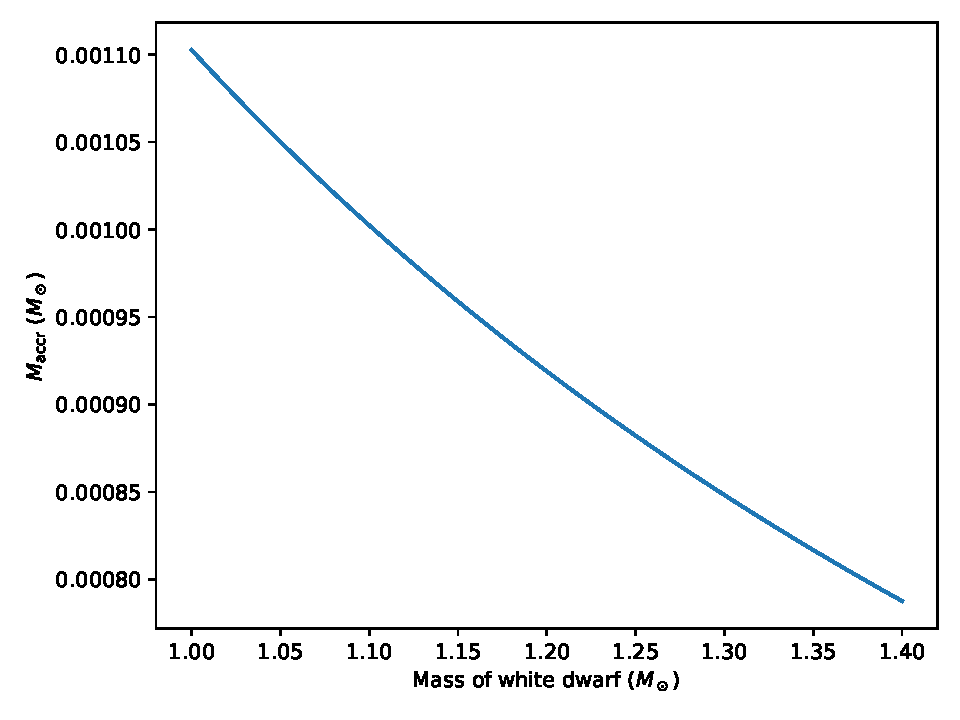
\includegraphics[width=0.75\textwidth]{proper_pressure_figure_1a}
        \end{center}
        With increasing white dwarf mass, the required mass to be accreted decreases. At higher white dwarf masses, the proper pressure is higher and therefore, nova explosions can happen earlier, i.e., at less total accreted mass.}
    \item {The accreted mass for a white dwarf of $1.2\,M_\odot$ required for it to explode is $9.2 \times 10^{-4}\,M_\odot$. At a radius of $0.01\,R_\odot$ the white dwarf will be 1.2 million times denser than the Sun.}
\end{enumerate}

\end{problem}

\begin{problem}{Recurrent Timescale for Classical Nova}
For the given mass accretion rates, the time scales for a nova to recur is between $9.2 \times 10^{7}$\,a and $9.2 \times 10^{3}$\,a. In order for recurring novae to explode in time intervals of 10\,a to 100\,a, such a system must either have a higher mass accretion rate or a lower required proper pressure for the thermonuclear runaway to occur.
\end{problem}

\begin{problem}{Classical Novae versus Type Ia Supernovae}
In both scenarios, matter from a main-sequence companion star is accreted onto a white dwarf. In the case of the SN-Ia however, the white dwarf's mass must already be close to the Chandrasekhar mass of around $1.4\,M_\odot$. Once that mass limit is exceeded, the star undergoes a core collapse and explodes as a supernova. For lower mass white dwarfs, this limit is not exceeded and the star accretes mass until a classical nova explosion takes place.
\end{problem}

\begin{problem}{Monte Carlo Error Propagation}
See solutions notebook online.
\end{problem}

\end{document}
